
% SECTION : logistic_regression {{{
\section{Logistic Regression}
\label{sec:logistic_regression}
\parindent=0em

% 	SUB-SECTION : hypothesis_equation {{{
\subsection{Hypothesis Equation}
\label{ssec:hypothesis_equation}
\parindent=0em

	Input / independant Variables : $ X \in \mathbb{R}^{m \times n}$
	Output / dependant Variables : $ y \in \{0,1\}$

\[ y \in \left\{ 0,1 \right\} \]

\[ y \in \left\{ 0,1,2,3, \ldots , n \right\} \]

\[
	\begin{array}{ l@{} l@{} } 
	\widehat{y} = \sigma(\theta_1 x_1 + \ldots + \theta_n x_n) 
	\end{array}
\]
\[
	\begin{array}{ l@{} l@{} }
		g(x)
		& =
		\frac{1}
		{
			1+e^
			{
				\left( - x \right)
			}
		}
	\end{array}
\]

 % sigmoid  {{{

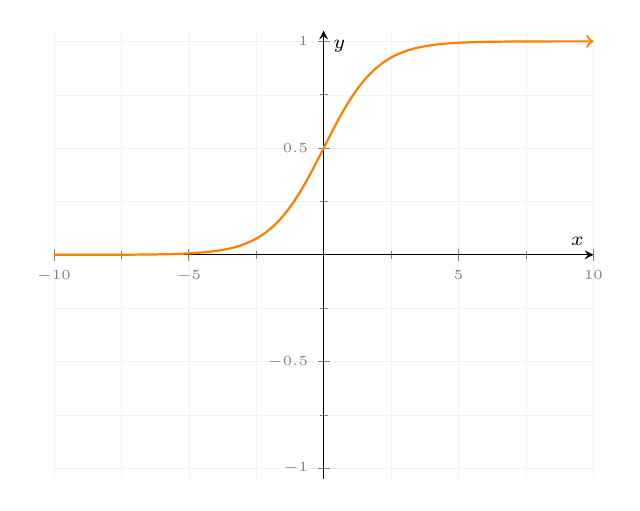
\begin{tikzpicture}
% axis settings {{{

\begin{axis}[
%	title          = graph_name,
	axis x line    = middle, % x-axis position
	axis y line    = middle, % y-axis position
	minor tick num = 1,      % num axis ticks
	grid           = both,
	grid style     =
	{
		line width=.1pt,
		draw=gray!10
	},
	xmax = 10,
	xmin = -10,
	ymax = 1.05, % 0.05 is to show the ->
	ymin = -1.05,
	tick label style = {
		font = \tiny,
		color = gray
	},
%	extra x ticks={3,1},
%	extra x tick labels={$\leftarrow$,$\rightarrow$},
%	extra y ticks={3,1},
%	extra y tick labels={$\leftarrow$,$\rightarrow$},
	legend style =
	{
		draw         = none, % remove legend bounding box
		font         = \tiny,
		legend pos   = outer north east,
		cells        = {anchor = west},
		fill         = gray,
		fill opacity = 0.4,
		text opacity = 1
	},
	xlabel       = {$\scriptstyle x$},
	ylabel       = {$\scriptstyle y$},
	xlabel style =
	{
		at     = {(ticklabel* cs:1)},
%		anchor = north west
	},
	ylabel style=
	{
		at     = {(ticklabel* cs:1)},
%		anchor = south west
	}
]
% }}}

\coordinate (O) at (0,0);

\addplot [
	domain=-10:10,
	no marks,
	samples=100,
	thick,
	orange,
	->
]
{1/(1+exp(-x)};
%\addlegendentry{$\frac{1}{1+e^{-x}}$};

\end{axis}
\end{tikzpicture}

% }}}

\[
\begin{array}{ l@{} l@{} l@{} }
	h_\theta(x)
	& = g(\theta_0 + \theta_1 x) 
	& =
	\frac{1}
	{
		1+e^
		{
			-
			\left(
				\theta_0 + \theta_1 x
			\right)
		}
	}
	\\
	h_\theta(X)
	& = g(\Theta^T X)
	& =
	\frac{1}
	{
		1+e^
		{
			-
			\left(
				\Theta^T X
			\right)
		}
	}
	\\
\end{array}
\]

\[
	\begin{array}{ l@{} l@{} }

	h_\theta(x) & = P(y=1|x;\theta)\\

	\end{array}
\]

\[
	\begin{array}{ l@{} l@{} }

	P(y=1|x;\theta) + P(y=0|x;\theta) & = 1 \\

	\end{array}
\]

\pagebreak
\subsectionend
% }}} END SUB-SECTION : hypothesis_equation
% 	SUB-SECTION : cost_function {{{
\subsection{Cost Function}
\label{ssec:cost_function}
\parindent=0em

Training set :

\[
	\begin{array}{ l@{} l@{} }
	\left\{
		\left( x^{(1)},y^{(1)} \right),
		\left( x^{(2)},y^{(2)} \right),
		\left( x^{(3)},y^{(3)} \right),
		\ldots
		\left( x^{(m)},y^{(m)} \right)
	\right\}
	\end{array}
\]

where we have m samples / examples for each data point x :

\[
	\begin{array}{ l@{} l@{} }
	\begin{bmatrix}
		x_0 \\
		x_1 \\
		\vdots \\
		x_n \\
		\end{bmatrix}
		_{1 \times(n+1)}
	\in \mathbb{R}^{n+1}
	\; , \;
	x_0 = {1}
	\; , \;
	y \in {0,1}
	\end{array}
\]



~\footnote{ Good explainer video : 
\href{ https://www.youtube.com/watch?v=XepXtl9YKwc }{https://www.youtube.com/watch?v=XepXtl9YKwc }
}



Which means that we have a new cost function $J(\theta)$:


\[
	\begin{array}{ l@{} l@{} }
	J(\theta)
	& =
	\dfrac{1}{m}
	\sum_{i=1}^m
	\left\{
		\mathrm{Cost}(h_\theta(x^{(i)}),y^{(i)})
	\right\}
	\\
	\mathrm{Cost}(h_\theta(x),y)
	& =
	\left\{
		\begin{array}{ l@{} l@{} } 
			-\log(h_\theta(x))
			\;
			& \text{if y = 1} 
			\\ 
			-\log(1-h_\theta(x))
			\;
			& \text{if y = 0} 
		\end{array}
	\right.  
	\end{array}
\]

\[
	\begin{array}{ l@{} l@{} }
		\mathrm{Cost}(h_\theta(x),y)
		&
		\left\{
		\begin{array}{ l@{} l@{} l@{} }
			& = 0
			& \text{ if } h_\theta(x) = y
			\\
			& \rightarrow \infty
			&\text{ if } y = 0
			\; \mathrm{and} \;
			h_\theta(x) \rightarrow 1
			\\
			& \rightarrow \infty
			& \text{ if } y = 1
			\; \mathrm{and} \;
			h_\theta(x) \rightarrow 0
			\\
		\end{array}
	\right.
	\end{array}
\]


	Case y = 1

	
% ln(x)  {{{

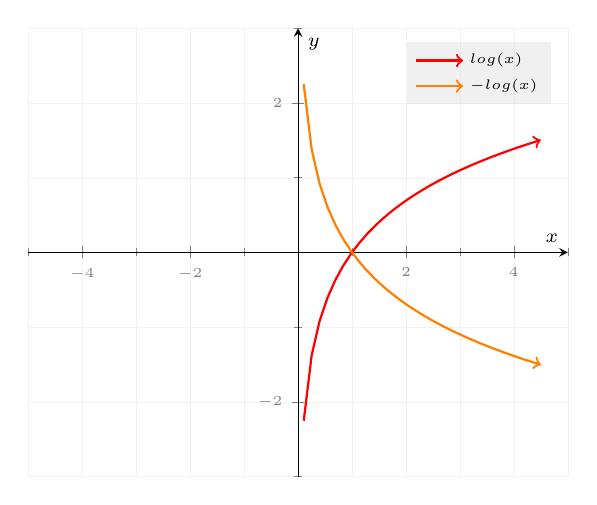
\begin{tikzpicture}
% axis settings {{{

\begin{axis}[
%	title          = graph_name,
	axis x line    = middle, % x-axis position
	axis y line    = middle, % y-axis position
	minor tick num = 1,      % num axis ticks
	grid           = both,
	grid style     =
	{
		line width = .1pt,
		draw       = gray!10
	},
	xmax      = 5,
	xmin      = -5,
	ymax      = 3,
	ymin      = -3,
	tick label style = {
		font  = \tiny,
		color = gray
	},
%	extra x ticks={3,1},
%	extra x tick labels={$\leftarrow$,$\rightarrow$},
%	extra y ticks={3,1},
%	extra y tick labels={$\leftarrow$,$\rightarrow$},
	legend style =
	{
		draw         = none, % remove legend bounding box
		font         = \tiny,
		legend pos   = north east,
		cells        = {anchor = west},
		fill         = gray!30,
		fill opacity = 0.4,
		text opacity = 1
	},
	xlabel       = {$\scriptstyle x$},
	ylabel       = {$\scriptstyle y$},
	xlabel style =
	{
		at     = {(ticklabel* cs:1)},
%		anchor = north west
	},
	ylabel style=
	{
		at     = {(ticklabel* cs:1)},
%		anchor = south west
	}
]
% }}}
\coordinate (O) at (0,0);

\addplot [
	domain=-10:4.5,
	samples=100,
	thick,
	red,
	->
]
{ln(x)};
\addlegendentry{$log(x)$};

\addplot [
	domain=-10:4.5,
	samples=100,
	thick,
	orange,
	->
]
{-ln(x)};
\addlegendentry{$-log(x)$};
\end{axis}
\end{tikzpicture}

% }}}
% ln(1-x)  {{{
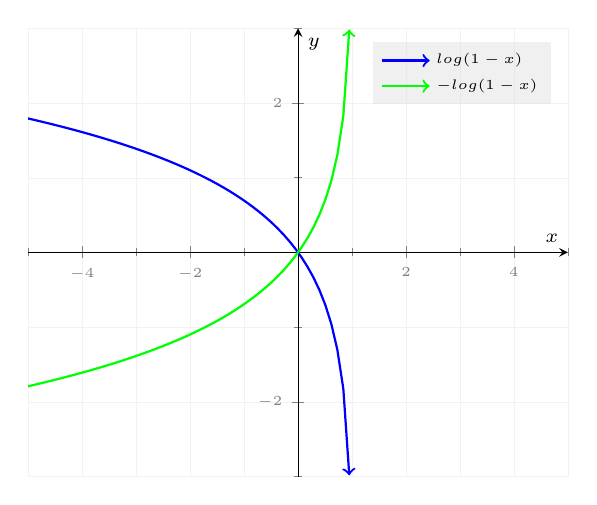
\begin{tikzpicture}
% axis settings {{{

\begin{axis}[
%	title          = graph_name,
	axis x line    = middle, % x-axis position
	axis y line    = middle, % y-axis position
	minor tick num = 1,      % num axis ticks
	grid           = both,
	grid style     =
	{
		line width = .1pt,
		draw       = gray!10
	},
	xmax      = 5,
	xmin      = -5,
	ymax      = 3,
	ymin      = -3,
	tick label style = {
		font  = \tiny,
		color = gray
	},
%	extra x ticks={3,1},
%	extra x tick labels={$\leftarrow$,$\rightarrow$},
%	extra y ticks={3,1},
%	extra y tick labels={$\leftarrow$,$\rightarrow$},
	legend style =
	{
		draw         = none, % remove legend bounding box
		font         = \tiny,
		legend pos   = north east,
		cells        = {anchor = west},
		fill         = gray!30,
		fill opacity = 0.4,
		text opacity = 1
	},
	xlabel       = {$\scriptstyle x$},
	ylabel       = {$\scriptstyle y$},
	xlabel style =
	{
		at     = {(ticklabel* cs:1)},
%		anchor = north west
	},
	ylabel style=
	{
		at     = {(ticklabel* cs:1)},
%		anchor = south west
	}
]
% }}}
\coordinate (O) at (0,0);

\addplot [
	domain=-10:0.95,
	samples=100,
	thick,
	blue,
	->
]
{ln(1-x)};
\addlegendentry{$log(1-x)$};

\addplot [
	domain=-10:0.95,
	samples=100,
	thick,
	green,
	->
]
{-ln(1-x)};
\addlegendentry{$-log(1-x)$};
\end{axis}
\end{tikzpicture}

% }}}
% ln(1-x)  {{{

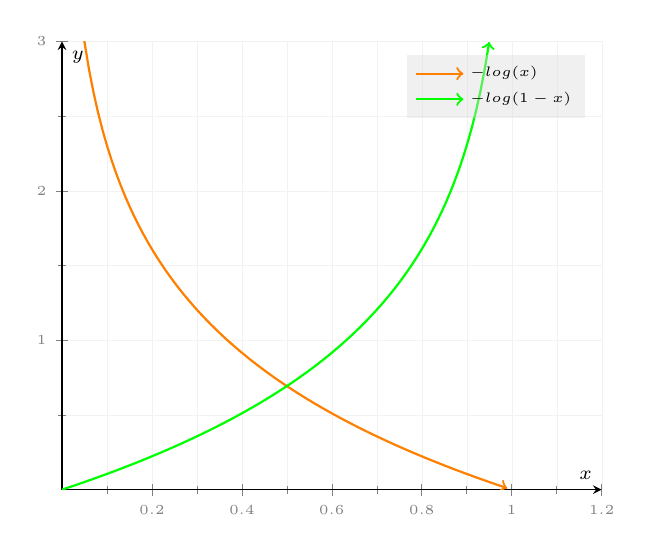
\begin{tikzpicture}
% axis settings {{{

\begin{axis}[
%	title          = graph_name,
	axis x line    = middle, % x-axis position
	axis y line    = middle, % y-axis position
	minor tick num = 1,      % num axis ticks
	grid           = both,
	grid style     =
	{
		line width = .1pt,
		draw       = gray!10
	},
	xmax      = 1.2,
	xmin      = 0,
	ymax      = 3,
	ymin      = 0,
	tick label style = {
		font  = \tiny,
		color = gray
	},
%	extra x ticks={3,1},
%	extra x tick labels={$\leftarrow$,$\rightarrow$},
%	extra y ticks={3,1},
%	extra y tick labels={$\leftarrow$,$\rightarrow$},
	legend style =
	{
		draw         = none, % remove legend bounding box
		font         = \tiny,
		legend pos   = north east,
		cells        = {anchor = west},
		fill         = gray!30,
		fill opacity = 0.4,
		text opacity = 1
	},
	xlabel       = {$\scriptstyle x$},
	ylabel       = {$\scriptstyle y$},
	xlabel style =
	{
		at     = {(ticklabel* cs:1)},
%		anchor = north west
	},
	ylabel style=
	{
		at     = {(ticklabel* cs:1)},
%		anchor = south west
	}
]
% }}}
\coordinate (O) at (0,0);

\addplot [
	domain=0:0.99,
	samples=100,
	thick,
	orange,
	->
]
{-ln(x)};
\addlegendentry{$-log(x)$};

\addplot [
	domain=0:0.95,
	samples=100,
	thick,
	green,
	->
]
{-ln(1-x)};
\addlegendentry{$-log(1-x)$};

\end{axis}
\end{tikzpicture}

% }}}

	Taking only the negative log from the graph and then using the interval
	only between $ 0 \leq x \leq 1$ , we get the following graph :

	Case y = 0
%	<img src="images/log_neg_interval.svg">
%	<img src="images/log_inv_neg_interval.svg">

\[
	\begin{array}{ l@{} l@{} l@{} } 
		\mathrm{Cost}(h_\theta(x),y)
		& = 0
		& \text{ if } h_\theta(x) = y 
		\\ 
		\mathrm{Cost}(h_\theta(x),y)
		& \rightarrow \infty
		&\text{ if } y = 0
		\; \mathrm{and} \;
		h_\theta(x) \rightarrow 1 
		\\ 
		\mathrm{Cost}(h_\theta(x),y)
		& \rightarrow \infty 
		& \text{ if } y = 1
		\; \mathrm{and} \;
		h_\theta(x) \rightarrow 0 
		\\ 
	\end{array}
\]

	\[
	\begin{array}{ l@{} l@{} } 
	J(\theta)
	& =
	\dfrac{1}{m}
	\sum_{i=1}^m
	\left\{
		\mathrm{Cost}(h_\theta(x^{(i)}),y^{(i)})
	\right\} 
	\\ 
	\mathrm{Cost}(h_\theta(x),y)
	& =
	\left\{ 
		\begin{array}{ l@{} l@{} } 
			-\log(h_\theta(x))
			\;
			& \text{if y = 1} 
			\\ 
			-\log(1-h_\theta(x))
			\;
			& \text{if y = 0} 
		\end{array}
	\right.  
	\\ 
	& = 
	-y\log(h_\theta(x))
	+
	(1-y)\log(1-h_\theta(x)) 
	\end{array}
\]


\[
	\begin{array}{ l@{} l@{} } 
	J(\theta)
	& =
	{ \displaystyle 
		\dfrac{1}{m}
		\sum_{i=1}^m
		\left\{
			\mathrm{Cost}(h_\theta(x^{(i)}),y^{(i)})
		\right\}
	}
	\\ 
	& =
	\dfrac{1}{m} 
	{ \displaystyle 
		\left(
			\sum_{i=1}^m
			\left\{
				-y^{(i)}\log(h_\theta(x^{(i)}))
				+
				(1-y^{(i)})\log(1-h_\theta(x^{(i)}))
			\right\}
		\right)
	} 
	\end{array}
\]

\[
	\begin{array}{ l@{} l@{} } 
		J(\theta)
		& =
		-
		\frac{1}{m}
		\cdot
		\sum_{i=1}^{m}
		\left\{
			y^{i}
			log(\widehat{y^{i}})
			+
			(1 - y^{i})
			log(1-\widehat{y^{i}})
		\right\}
	\end{array}
\]

\pagebreak
\subsectionend
% }}} END SUB-SECTION : cost_function
% 	SUB-SECTION : gradient_descent {{{
\subsection{Gradient Descent}
\label{ssec:gradient_descent}
\parindent=0em

\[
	\begin{array}{ l@{} l@{} }
		\nabla J(\Theta)
		& =
		\left\langle
		  {\displaystyle \frac{\partial}{\partial \theta_0} J(\Theta)}
		, {\displaystyle \frac{\partial}{\partial \theta_1} J(\Theta)}
		, {\displaystyle \frac{\partial}{\partial \theta_2} J(\Theta)}
		\ldots
		, {\displaystyle \frac{\partial}{\partial \theta_m} J(\Theta)}
		\right\rangle
		\\
	\end{array}
\]


\[
	\begin{array}{ l@{} l@{} }
\sigma(x)             & = \frac{1}{1+e^{-x}} \\
\frac{d}{dx}\sigma(x) & = \frac{d}{dx} \left(  \frac{1}{1+e^{-x} } \right) \\
                      & = \frac{0 \cdot(1+e^{-x}) - (-e^{-x}) \cdot 1}{ ( 1+e^{-x} ) ^2} \text{$\hspace{46 mm}$Quotient rule}\\
                      & = \frac{e^{-x}}{ ( 1+e^{-x} ) ^2}  \\
                      & = \frac{(1+e^{-x}) -1 }{ ( 1+e^{-x} ) ^2} \\
                      & = \frac{ (1+e^{-x})}{ ( 1+e^{-x} ) ^2}  - \left( \frac{1}{1+e^{-x}} \right)^2\\
                      & = \frac{1}{1+e^{-x}}  - \left( \frac{1}{1+e^{-x}} \right)^2\\
                      & = \sigma (x) - \sigma(x)^2\\
\sigma^{'} (x)        & = \sigma(x)(1-\sigma(x))
	\end{array}
\]


We also have the following :
\[
	\begin{array}{ l@{} l@{} } 
		h_\theta(\Theta^T x)
		= \sigma(\Theta^Tx)
		& = \frac{1}{1+e^{-\Theta^T x}} \\ 
	\end{array}
\]

\[
\begin{array}{ l@{} l@{} l@{} l@{} } 
		P(y^{(i)} = 1 | x^{(i)} ; \theta)
		& = h_\theta(x)
		& = \sigma(x)
		& = \frac{1}{1+e^{-x}}
		\\ 
		P(y^{(i)} = 0 | x^{(i)} ; \theta)
		& = 1 - h_\theta(x)
		& = 1 - \sigma(x)
		& = 1 - \frac{1}{1+e^{-x}}
		\\ 
	\end{array}
\]

This gives us the overall likelihood of any outcome y given x and theta as :

\[
\begin{array}{ l@{} l@{} l@{} } 
		L(\theta) 
		& = P(y^{(i)}| x^{(i)} ; \theta)
		& = h(x^{(i)})^{y^{(i)}} \cdot ( 1 - h(x^{(i)}))^{1 - y^{(i)}} 
	\end{array}
\]

overall i's

\[
	\begin{array}{ l@{} l@{} }
	L(\theta) & =
	{ \displaystyle \prod_{i=1}^{m} }
	\left\{
		h
		\left(x^{(i)}\right)
		^{
			\left(
				y^{(i)}
			\right)
		}
		\cdot
		\left(
			1 - h(x^{(i)})
		\right)
		^{
			\left(
				1 - y^{(i)}
			\right)
		}
	\right\}
	\\
	\log(L(\theta)) & = \mathscr{L}(\theta) \\ 
	\mathscr{L}(\theta)
	& =
	\log \left( 
	{ \displaystyle \prod_{i=1}^{m} }
	\left\{
		h
		\left(x^{(i)}\right)
		^{
			\left(
				y^{(i)}
			\right)
		} 
		\cdot 
		\left(
			1 - h(x^{(i)})
		\right)
		^{
			\left(
				1 - y^{(i)}
			\right)
		} 
	\right\} 
	\right) 
	\\ 
	& = 
	{ \displaystyle \sum_{i=1}^{m} } \left\{ 
		\log \left( 
			h
			\left(x^{(i)}\right)
			^{
				\left(
					y^{(i)}
				\right)
			} 
			\cdot 
			\left(
				1 - h(x^{(i)})
			\right)
			^{
				\left(
					1 - y^{(i)}
				\right)
			} 
		\right) 
	\right\} 
	\\ 
	& = 
	{ \displaystyle \sum_{i=1}^{m} } \left\{ 
		\log \left( 
			h
			\left(x^{(i)}\right)
			^{
				\left(
					y^{(i)}
				\right)
			} 
		\right) 
		+ 
		\log \left( 
			\left(
				1 - h(x^{(i)})
			\right)
			^{
				\left(
					1 - y^{(i)}
				\right)
			} 
		\right) 
	\right\} 
	\\ 
	& = 
	{ \displaystyle \sum_{i=1}^{m} } \left\{ 
		\left(
			y^{(i)}
		\right) 
		\cdot 
		\log \left( 
		h \left(
			x^{(i)}
		\right) 
		\right) 
		+ 
		\left(
			1 - y^{(i)}
		\right) 
		\cdot 
		\log \left( 
		\left(
			1 -
			h \left(
				x^{(i)}
			\right) 
		\right) 
		\right) 
	\right\} 
	\end{array}
\]

We want to maximize the likelihood so we take the derivative :


\[
	\begin{array}{ l@{} l@{} r@{} } 
	{ \displaystyle \frac{\partial}{\partial \theta}}
	\mathscr{L}(\theta) 
	& = 
	{ \displaystyle \frac{\partial}{\partial \theta}}
	\left(
		{ \displaystyle \sum_{i=1}^{m} } \left\{ 
			\left(
				y^{(i)}
			\right) 
			\cdot 
			\log \left( 
			h \left(
				x^{(i)}
			\right) 
			\right) 
			+ 
			\left(
				1 - y^{(i)}
			\right) 
			\cdot 
			\log \left( 
			\left(
				1 -
				h \left(
					x^{(i)}
				\right) 
			\right) 
			\right) 
		\right\}
	\right) 
	\\ 
	& = 
	{ \displaystyle \frac{\partial}{\partial \theta}}
	\left(
		{ \displaystyle \sum_{i=1}^{m} } \left\{ 
			\left(
				y^{(i)}
			\right) 
			\cdot 
			\log \left( 
			\sigma \left(
				x^{(i)}
			\right) 
			\right) 
			+ 
			\left(
				1 - y^{(i)}
			\right) 
			\cdot 
			\log \left( 
			\left(
				1 -
				\sigma \left(
					x^{(i)}
				\right) 
			\right) 
			\right) 
		\right\}
	\right) 
	\\ 
	& = 
	{ \displaystyle \sum_{i=1}^{m} } \left\{ 
		\left(
			y^{(i)}
		\right) 
		\cdot 
		{ \displaystyle \frac{\partial}{\partial \theta}} \left( 
			\log \left( 
			\sigma \left(
				x^{(i)}
			\right) 
			\right) 
		\right) 
		+ 
		\left(
			1 - y^{(i)}
		\right) 
		\cdot 
		{ \displaystyle \frac{\partial}{\partial \theta}} \left( 
			\log \left( 
			\left(
				1 -
				\sigma \left(
					x^{(i)}
				\right) 
			\right) 
		\right) 
	\right\} 
	\right) 
	\\ 
	& = 
	{ \displaystyle \sum_{i=1}^{m} } \left\{ 
		\left(
			y^{(i)}
		\right) 
		\cdot 
		\left( 
			{ \displaystyle
			\frac
				{
					1
				}
				{
					\sigma \left( x^{(i)} \right)
				}
			} 
			\cdot 
			\sigma \prime \left( x^{(i)} \right) 
		\right) 
		+ 
		\left( 1 - y^{(i)} \right) 
		\cdot 
		\left( 
			{ \displaystyle
			\frac
				{
					1
				}
				{
					1 - \sigma \left( x^{(i)} \right)
				}
			} 
			\cdot 
			- \sigma \prime \left( x^{(i)} \right) 
		\right) 
	\right\} 
	& \text{Chain Rule} 
	\\ 
	& = 
	\end{array}
\]

Gradient Descent

\[
	\begin{array}{ l@{} l@{} } 
		\frac{\partial}{\partial \theta_0} J(\Theta)
		& =
		\left(
			\frac{1}{m}
			\cdot
			\sum_{i=1}^m \left\{
					\left(
						h_\theta(x^{(i)}) - y^{(i)}
					\right)^{2}
					\cdot
					x_{0}^{(i)}
			\right\}
		\right) 
		\\ 
		\frac{\partial}{\partial \theta_j} J(\Theta)
		& =
		\left(
			\frac{1}{m} \cdot
			\sum_{i=1}^m \left\{
				\left(
					h_\theta(x^{(i)}) - y^{(i)}
				\right)^{2}
				\cdot
				x_{j}^{(i)}
			\right\}
		\right) 
		+ 
		\frac{\lambda}{m}\cdot \theta_j 
		\\ 
	\end{array}
\]

The second sum, 
\( \frac{\lambda}{2m}
   \sum_{j = 1}^{n} {\theta_{j}^{2}} \)
means to explicitly exclude the bias term, $\theta_0$. i.e. the $\theta$
vector is indexed from 0 to n (holding n+1 values, $\theta_0$ through
$\theta_n$), and this sum explicitly skips $\theta_0$, by
running from 1 to n, skipping 0. Thus, when computing the equation, we should
continuously update the two following equations:

	\[
	\begin{array}{ l@{} l@{} l@{} l@{} } 
		\theta_0
		& := &
		\theta_0
		- \alpha
		\cdot
		\left(
		\frac{1}{m}
		\cdot 
			\sum_{i=1}^m
			\left\{
				\left(
					h_\theta(x^{(i)}) - y^{(i)}
				\right)^{2}
				\cdot
				x_{0}^{(i)}
			\right\}
		\right) 
		\hspace{0.5cm} & \text{for} \; j = 0 
		\\ 
		\theta_j
		& := &
		\theta_j
		- \alpha
		\cdot
		\left(
		\frac{1}{m}
		\cdot 
			\sum_{i=1}^m
			\left\{
				\left(
					h_\theta(x^{(i)}) - y^{(i)}
				\right)^{2}
				\cdot
				x_{j}^{(i)}
				+
				\left(
					\frac{\lambda}{m}\cdot \theta_j
				\right)
			\right\}
		\right) 
		\hspace{0.5cm} & \text{for} \; j = 1,2, \ldots , n 
		\\ 
		& :=
		& \theta_j
		\cdot
		(1 - \alpha \cdot \frac{\lambda}{m})
		-
		\alpha
		\cdot
		\left(
		\frac{1}{m}
		\cdot 
			\sum_{i=1}^m
			\left\{
				\left(
					h_\theta(x^{(i)}) - y^{(i)}
				\right)^{2}
				\cdot
				x_{j}^{(i)} 
			\right\}
		\right) 
		\\ 
		\end{array}
	\]

Using gradient descent the gradient vector is :

\[
	\begin{array}{ l@{} l@{} } 
		\nabla J
		& = 
		\begin{bmatrix} 
			\frac{\partial J(\theta_1)}{\partial \theta_1}  \\ 
			\frac{\partial J(\theta_2)}{\partial \theta_2}  \\ 
			\vdots \\ 
			\frac{\partial J(\theta_k)}{\partial \theta_k}  \\ 
		\end{bmatrix} 
	\end{array}
\]

\[
	\begin{array}{ l@{} l@{} } 
		\frac{\partial}{\partial \theta_0} J(\theta_1)
		& =
		-
		\frac{1}{m}
		\cdot 
		\sum_{i=1}^m
		\left\{
			\left(
				y^{i} - \widehat{y^{i}}
			\right)
			\cdot
			x_{1}^{i}
		\right\} 
	\end{array}
\]


\pagebreak
\subsectionend
% }}} END SUB-SECTION : gradient_descent
% 	SUB-SECTION : update_rule {{{
\subsection{Update Rule}
\label{ssec:update_rule}
\parindent=0em

\[
	\begin{array}{ l@{} l@{} } 
	\theta_{new} = \theta_{prev} - \eta \nabla J 
	\end{array}
\]

\subsectionend
% }}} END SUB-SECTION : update_rule

% 	SUB-SECTION : extra {{{
\subsection{Extra}
\label{ssec:extra}
\parindent=0em

% 		SUB-SUB-SECTION : multiclass_classification {{{
\subsubsection{Multiclass Classification}
\label{sssec:multiclass_classification}
\parindent=0em

		\[
			\begin{array}{ l@{} l@{} }
				h_\theta^{(i)}(x) = P(y=i|x;\theta) \; , \; 1 \leq i \leq k , k
				\in \mathbb{N}
			\end{array}
		\]

		
		\[
			\begin{array}{ l@{} l@{} }
				\max\limits_i h_\theta^{(i)}(x) &
			\end{array}
		\]

\pagebreak
\subsubsectionend
% }}} END SUB-SUB-SECTION : multiclass_classification
% 		SUB-SUB-SECTION : overfitting {{{
\subsubsection{Overfitting}
\label{sssec:overfitting}
\parindent=0em

	\[
		\begin{array}{ l@{} l@{} }


			J(\theta)
			= \frac{1}{2m}
			\sum_{i=1}^m
			\left\{
				\left(
					h_\theta(x^{(i)}) - y^{(i)}
				\right)^{2}
			\right\}

			\approx 0


		\end{array}
	\]

\pagebreak
\subsubsectionend
% }}} END SUB-SUB-SECTION : overfitting
% 		SUB-SUB-SECTION : regularization {{{
\subsubsection{Regularization}
\label{sssec:regularization}
\parindent=0em


\[
	\begin{array}{ l@{} l@{} } 
		\frac{1}{2} \cdot
		\frac{1}{m} \cdot 
		\lambda \cdot
		\sum_{j = 1}^{n}
		\left\{
			{\theta_{j}^{2}}
		\right\} 
	\end{array}
\]

$\lambda$ is called the regularization parameter. Its job is to control the
tradeoff between two different goals. The first goal is to actually fit the
training data well. This is done by our original cost function $J(\theta)$. The
second goal is to keep the parameters small. 

\[
	\begin{array}{ l@{} l@{} } 
		J(\theta)
		=
		\left( 
		\frac{1}{2}
		\cdot
		\frac{1}{m}
		\cdot 
			\left(
				\sum_{i=1}^m
				\left\{
					\left(
						h_\theta(x^{(i)}) - y^{(i)}
					\right)^{2}
				\right\}
			\right) 
			+
			\left( 
				\frac{1}{2} \cdot
				\frac{1}{m} \cdot 
				\lambda \cdot
				\sum_{j = 1}^{n}
				\left\{
					{\theta_{j}^{2}}
				\right\}
			\right)
		\right) 
	\end{array} 
\]

\[
	\begin{array}{ l@{} l@{} } 
		\min\limits_\theta
		J(\theta)
		=
		\frac{1}{2}
		\cdot
		\frac{1}{m}
		\cdot
		\left(
			\left(
				\sum_{i=1}^m
				\left\{
					\left(
						h_\theta(x^{(i)}) - y^{(i)}
					\right)^{2}
				\right\}
			\right) 
			+
			\left( 
				\frac{1}{2} \cdot
				\frac{1}{m} \cdot
				\lambda \cdot
				\sum_{j = 1}^{n}
				\left\{
					{\theta_{j}^{2}}
				\right\}
			\right)
		\right) 
	\end{array} 
\]


\subsubsectionend
% }}} END SUB-SUB-SECTION : regularization

\pagebreak
\subsectionend
% }}} END SUB-SECTION : extra

%\sectionend
% }}} END SECTION : logistic_regression
